\section{Assignment 4}

\subsection{Image analysis using morphological operators}

2D image analysis can be carried out with the use of morphological operators. Image closing and opening let us remove the background of pictures and isolate the objects within them. More complex operations can then be carried out, inferring for example geometric information on the shapes produced.

\subsubsection{Example 1}

Background removed by opening with a structuring element in the shape of a disk of size 65. Shapes improved by image closing with a structuring element in the shape of a disk of size 25 and by filling holes. Noise removed after image binarization with area opening, removing all shapes with fewer than 50 pixels.

Classification used the 'Circularity' property to distinguish between coins and USB stick, as well as the 'MajorAxis' and 'MinorAxis' properties, which were averaged to compute the radius of the coins to detect which was smaller and which was bigger.

\begin{figure}[h]
\centering
\begin{minipage}{0.45\textwidth}
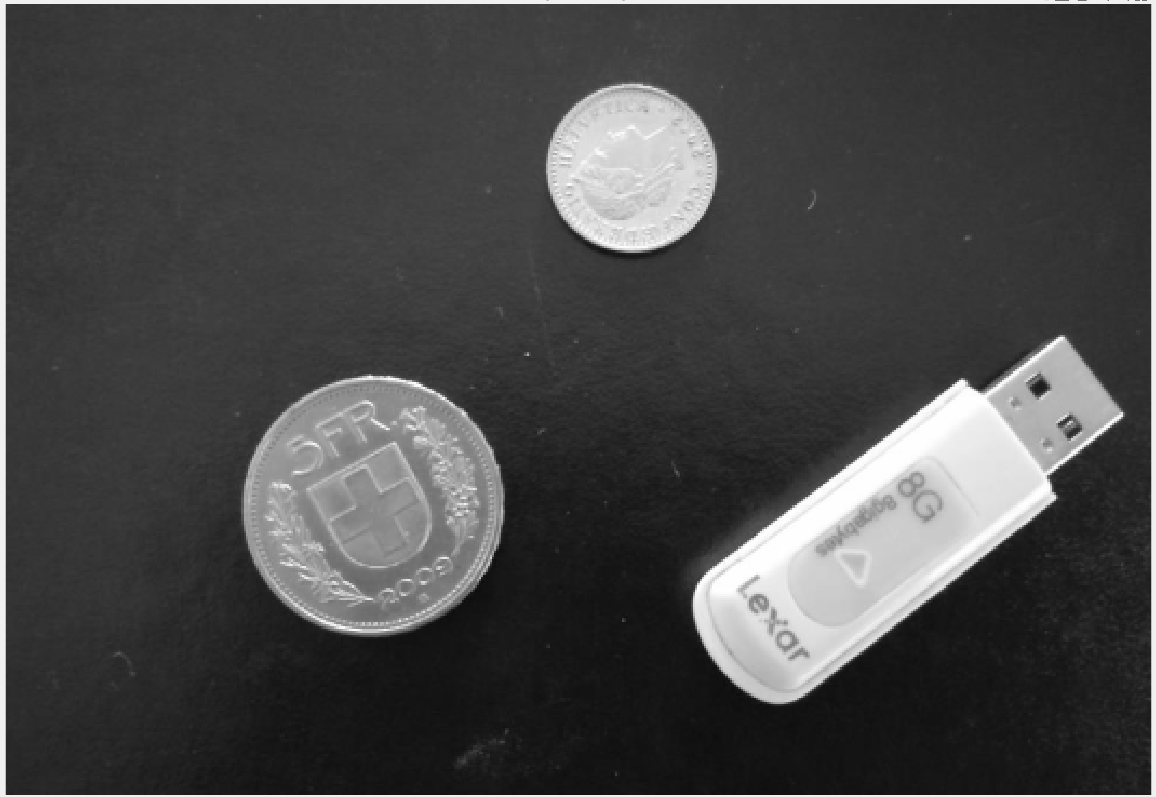
\includegraphics[keepaspectratio,width=0.9\textwidth]{4_coins_original}
\end{minipage}
\begin{minipage}{0.45\textwidth}
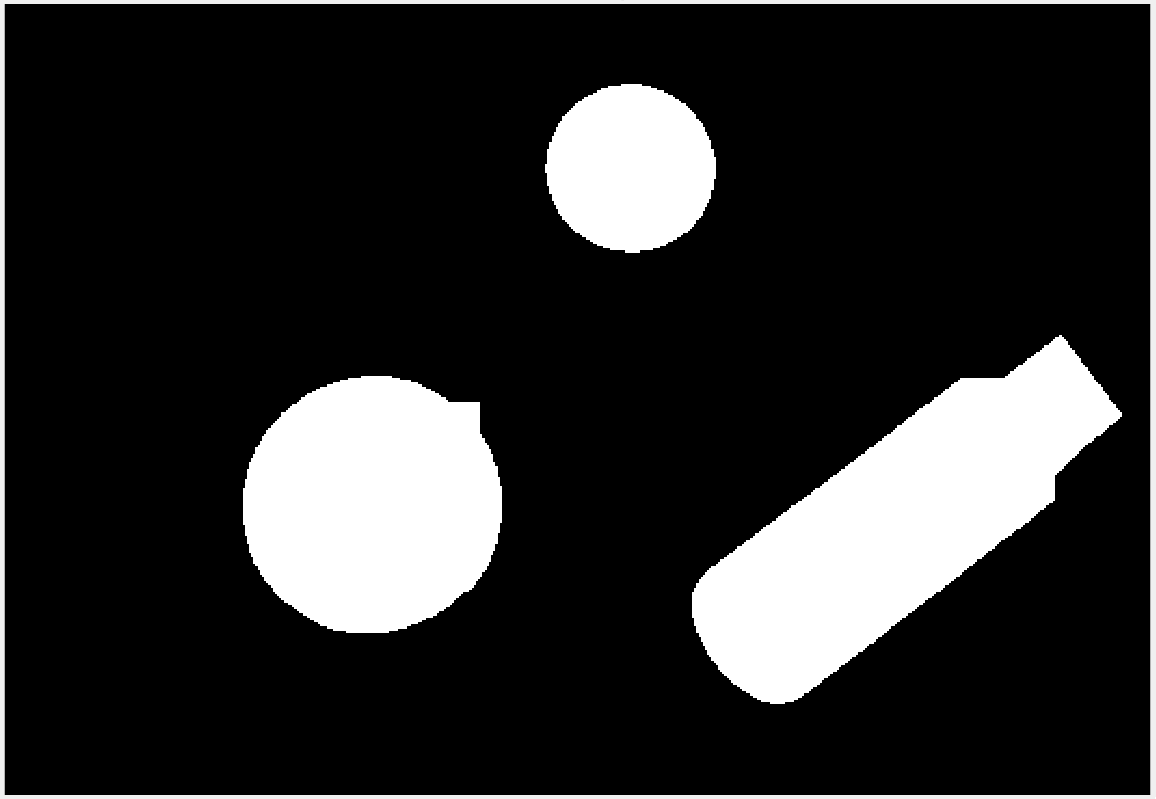
\includegraphics[keepaspectratio,width=0.9\textwidth]{4_coins_shapes}
\end{minipage}
\caption{Original image (left) vs extracted shapes (right).}
\end{figure}
\begin{figure}[h]
\centering
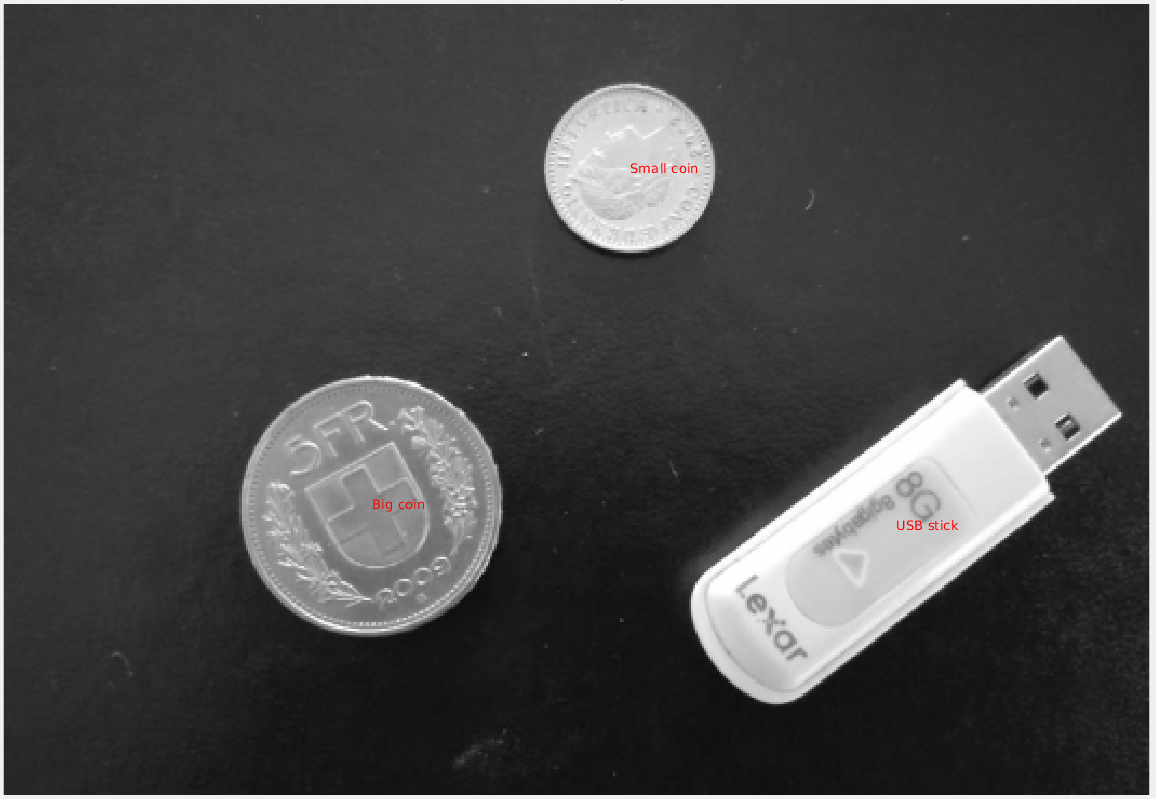
\includegraphics[keepaspectratio,width=0.5\textwidth]{4_coins_labels}
\caption{Labeled image.}
\end{figure}

\newpage

\subsubsection{Example 2}

Background removed by opening with a structuring element in the shape of a disk of size 65. Shapes improved by image closing with a structuring element in the shape of a disk of size 25 and by filling holes. Noise removed after image binarization with area opening, removing all shapes with fewer than 50 pixels.

Classification used the 'Circularity' property to distinguish between washers and bolts. The 'MajorAxis' and 'MinorAxis' properties were averaged to compute the outer radius of the washers, on which a quintic polynomial was fit to determine the relation with the actual inner diameter. For the bolts, the 'Orientation' property was used to align the shapes vertically, so that the bottom part of them, which contains the threaded part, could be extracted. On the extracted shapes, the 'MajorAxis' and 'MinorAxis' properties were extracted and used to fit cubic polynomials to determine, respectively, the bolt length and diameter.

\begin{figure}[h]
\centering
\begin{minipage}{0.3\textwidth}
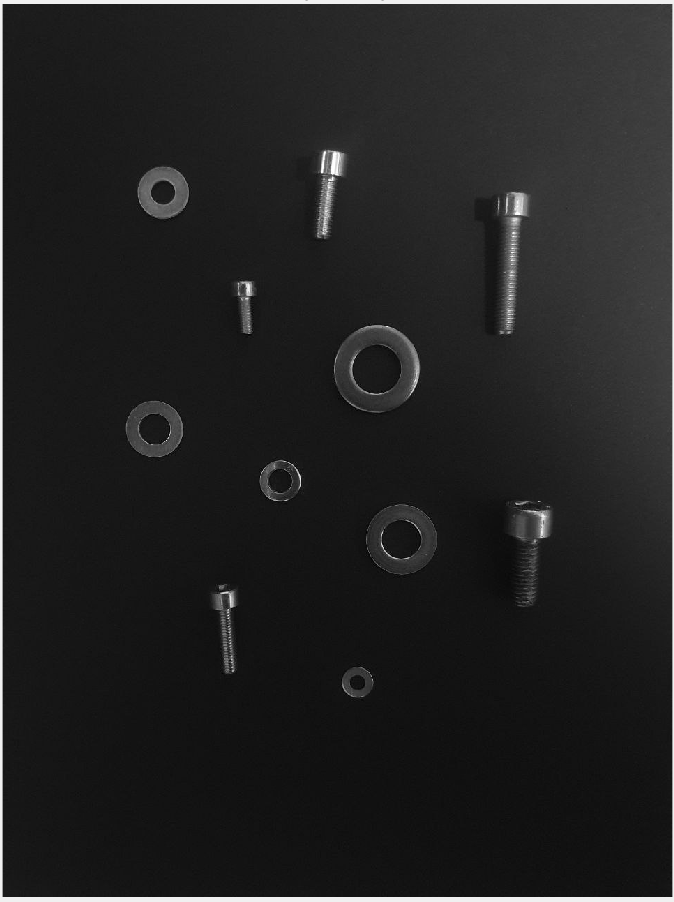
\includegraphics[keepaspectratio,width=0.9\textwidth]{4_nuts_original}
\end{minipage}
\begin{minipage}{0.3\textwidth}
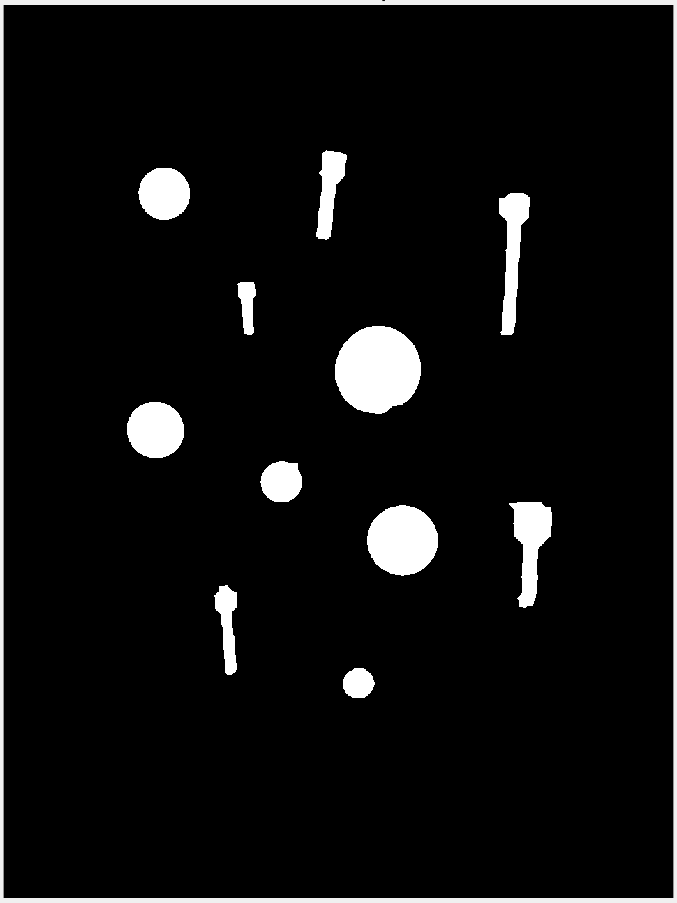
\includegraphics[keepaspectratio,width=0.9\textwidth]{4_nuts_shapes}
\end{minipage}
\begin{minipage}{0.3\textwidth}
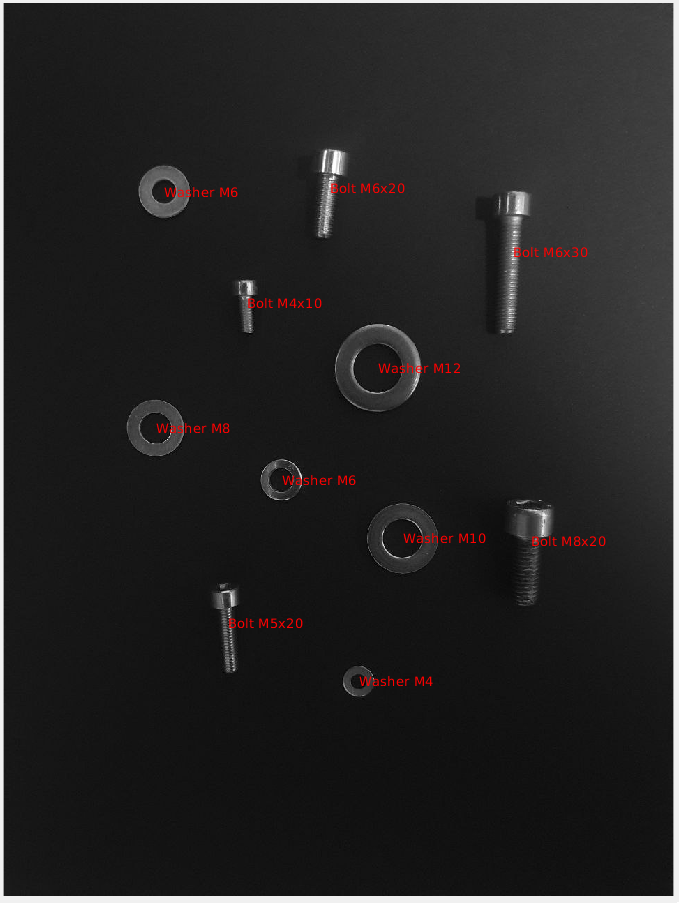
\includegraphics[keepaspectratio,width=0.9\textwidth]{4_nuts_labels}
\end{minipage}
\caption{Original image (left) vs extracted shapes (middle) vs labels (right).}
\end{figure}